\documentclass{llncs}
\usepackage[utf8]{inputenc}
\usepackage[T1]{fontenc}
\usepackage[english]{babel}
\usepackage{lmodern}
\usepackage{makeidx}
\usepackage{fancyhdr}
\usepackage{pstricks}
\usepackage{graphicx}
\usepackage{subfigure}
%\usepackage{a4wide} 
\usepackage{amsmath}
\usepackage{amssymb}
\usepackage{amsfonts}
%\usepackage{amsthm}
\usepackage{array}
\usepackage{tikz}
\usepackage{color}
\usepackage{dsfont}
\usepackage{hyperref}
\usepackage{mathtools}
\usepackage{stmaryrd}
\usepackage{xparse} 

\definecolor{myviolet}{RGB}{193,170,222}
%\usepackage{graphicx}
%
\usetikzlibrary{calc,trees,positioning,arrows,chains,shapes.geometric,%
    decorations.pathreplacing,decorations.pathmorphing,shapes,%
    matrix,shapes.symbols}

\tikzset{
>=stealth',
  punktchain/.style={
    rectangle, 
    rounded corners, 
    % fill=black!10,
    draw=black, very thick,
    text width=10em, 
    minimum height=3em, 
    text centered, 
    on chain},
    testr/.style={
    rectangle, 
    rounded corners, 
    % fill=black!10,
    draw=gray, very thick,

    text width=10em, 
    minimum height=3em, 
    text centered, 
    on chain},
  machain/.style={
    rectangle, 
    rounded corners, 
    % fill=black!10,
    draw=black, very thick,
    text width=0.8\textwidth, 
    minimum height=3em, 
    text centered, 
    on chain},
  line/.style={draw, thick, <-},
  element/.style={
    tape,
    top color=white,
    bottom color=blue!50!black!60!,
    minimum width=8em,
    draw=blue!40!black!90, very thick,
    text width=10em, 
    minimum height=3.5em, 
    text centered, 
    on chain},
  every join/.style={->, thick,shorten >=1pt},
  decoration={brace},
  tuborg/.style={decorate},
  tubnode/.style={midway, right=2pt},
}

%% figures vs text
\renewcommand{\topfraction}{.85}
\renewcommand{\bottomfraction}{.7}
\renewcommand{\textfraction}{.15}
\renewcommand{\floatpagefraction}{.66}
\renewcommand{\dbltopfraction}{.66}
\renewcommand{\dblfloatpagefraction}{.66}
\setcounter{topnumber}{9}
\setcounter{bottomnumber}{9}
\setcounter{totalnumber}{20}
\setcounter{dbltopnumber}{9}

%% remark macros
\newcommand{\eloremark}[1]{\textcolor{violet}{#1}}
\newcommand{\hugremark}[1]{\textcolor{cyan}{#1}}
\newcommand{\htremark}[1]{\textcolor{blue}{#1}}
\newcommand{\Zset}{\mathbb{Z}}
\newcommand{\imgtop}{\mathds{1}}

%% math macros
%\newtheorem{definition}{Definition}
%newtheorem{theorem}{Theorem}

\providecommand{\RW}{\ensuremath{W^r}}
\providecommand{\myceil}[1]{\ensuremath{\left\lceil #1 \right\rceil}}
\providecommand{\myfloor}[1]{\ensuremath{\left \lfloor #1 \right \rfloor}}
\DeclareMathOperator{\MSD}{\ensuremath{\text{MSD}}}

\DeclarePairedDelimiter\ceil{\lceil}{\rceil}
\DeclarePairedDelimiter\floor{\lfloor}{\rfloor}

\DeclarePairedDelimiterX{\Iintv}[1]{\llbracket}{\rrbracket}{\iintvargs{#1}}
\NewDocumentCommand{\iintvargs}{>{\SplitArgument{1}{,}}m}
{\iintvargsaux#1} %
\NewDocumentCommand{\iintvargsaux}{mm} {#1\mkern1.5mu..\mkern1.5mu#2}

\DeclareMathOperator*{\argmax}{arg\,max}
\DeclareMathOperator*{\argmin}{arg\,min}

\begin{document}


\title{Spherical fluorescent particle segmentation and tracking in 3D confocal microscopy}

\author{\'{E}lodie Puybareau\inst{1,2} \and Edwin Carlinet\inst{1} \and Alessandro Benfenati\inst{2} \and Hugues Talbot\inst{2,3}}

\institute{
EPITA Research and Development,
14-16 rue Voltaire, F-94276 Le Kremlin-Bicetre
\and
Université Paris-Est, ESIEE Paris, 2 boulevard Blaise-Pascal, F-93162 Noisy-le-Grand
\and
CentraleSupelec, Centre de Vision Numérique, INRIA équipe OPIS, 3 rue Joliot-Curie, F-91190
Gif-sur-Yvette.
}

\maketitle

\begin{abstract}
Spherical fluorescent particle are micrometer-scale spherical beads used in various areas of physics, chemistry or biology as markers associated
with local physical media. They are useful for example in fluid dynamics to characterize flows, diffusion coefficients, viscosity or temperature; they 
are used in cells dynamics to estimate mechanical strain and stress at the micrometer scale. In order to estimate these physical measurements, tracking these
particles is necessary. Numerous approaches and existing packages, both open-source and proprietary are available to achieve tracking with a high degree of precision in 2D. However,
little such software is available to achieve tracking in 3D. One major difficulty is that 3D confocal microscopy acquisition is not typically fast enough to assume
that the beads are stationary during the whole 3D scan. As a result, beads may move between planar scans. Classical approaches to 3D segmentation may yield objects are not spherical.
In this article, we propose a 3D bead segmentation that deals with this situation. 

\keywords{Segmentation, shaping.}
\end{abstract}

\section{Introduction}\label{sec:Introduction}
The use of fluorescent beads as physical markers is common in many research problems and applications related to fluid mechanics~\cite{park2005temperature}, rheology~\cite{PGDG:Polymers:1979}, and cell biology~\cite{wang1993mechanotransduction}.

Spherical bead tracking in confocal microscopy is a classical and well-studied problem in image analysis. Recently, an ISBI challenge was organized to compare state-of-the-art bead segmentation and tracking methods~\cite{chenouard2014objective}. However, this very challenge has exhibited a number of shortcomings.

First among them is the common assumption that beads are very small, similar in diameter to the optical limit of resolution of the microscope, i.e. 0.2-0.4$\mu$m. In reality, beads can be much larger than this. 1-2$\mu$m diameters are commonly used. This is due to the fact that larger beads are less expensive, more visible and better adapted to some problems, for example when the surface of the bead needs to be activated. In particular, tracking of very small beads is difficult when there are many beads. Due to their larger dimension, a more precise location of their center is also possible, whereas smaller beads are typically only made of a few pixels and so a precise location of their center is imprecise.

A second assumption is that since beads are expected to be very small, they are located in a single plane and are so acquired in a single pass. Unfortunately, larger beads span several planes and need to be acquired over several scans, which takes time.

Thirdly, a common assumption is that scanning time is negligible compared with the studied motion. This is often true in mechanical cell studies. However, in fluid analysis, beads are subjected to Brownian motion~\cite{Brown:Motion:1828} and can move significantly even in the absence of flow. This is a problem even during a single 3D acquisition since a bead can visible move as the confocal scan is taking place.

In this article, we study and propose solutions for comparatively large bead segmentation and tracking. Due to Brownian motion, tracking must take place both at the intra and inter-volume level. We present an application where we measure the diffusion coefficient of the Brownian motion. This is useful for measuring viscosity or temperature in fluid media~\cite{puybareau2017morphological}.


\section{Particle tracking}\label{sec:tracking}
Our objective is to track relatively large beads (0.8-2$\mu$m in diameter) in 3D confocal microscopy. We do not assume that the diameter is known precisely. Typically most bead production processes allow a standard deviation of $\pm$ 10\%. Traditional confocal microscopy proceeds by scanning a 3D volume slice-by-slice. Scanning a small area of a single slice, such as the few lines that may include a bead, is fast enough that the intersection of a scanning plane with any bead can be assumed to be a disk. However, scanning a whole slice can be slow, and so the particle may move slightly in between slice acquisition. 

We do not assume that the particle forms a perfect sphere. We do assume that deviations from the sphere are relatively small. We also assume that the slice separation is small enough so that each bead is scanned multiple times. This is typically an adjustable parameter of the microscope.


\begin{figure}[htb]
\centering
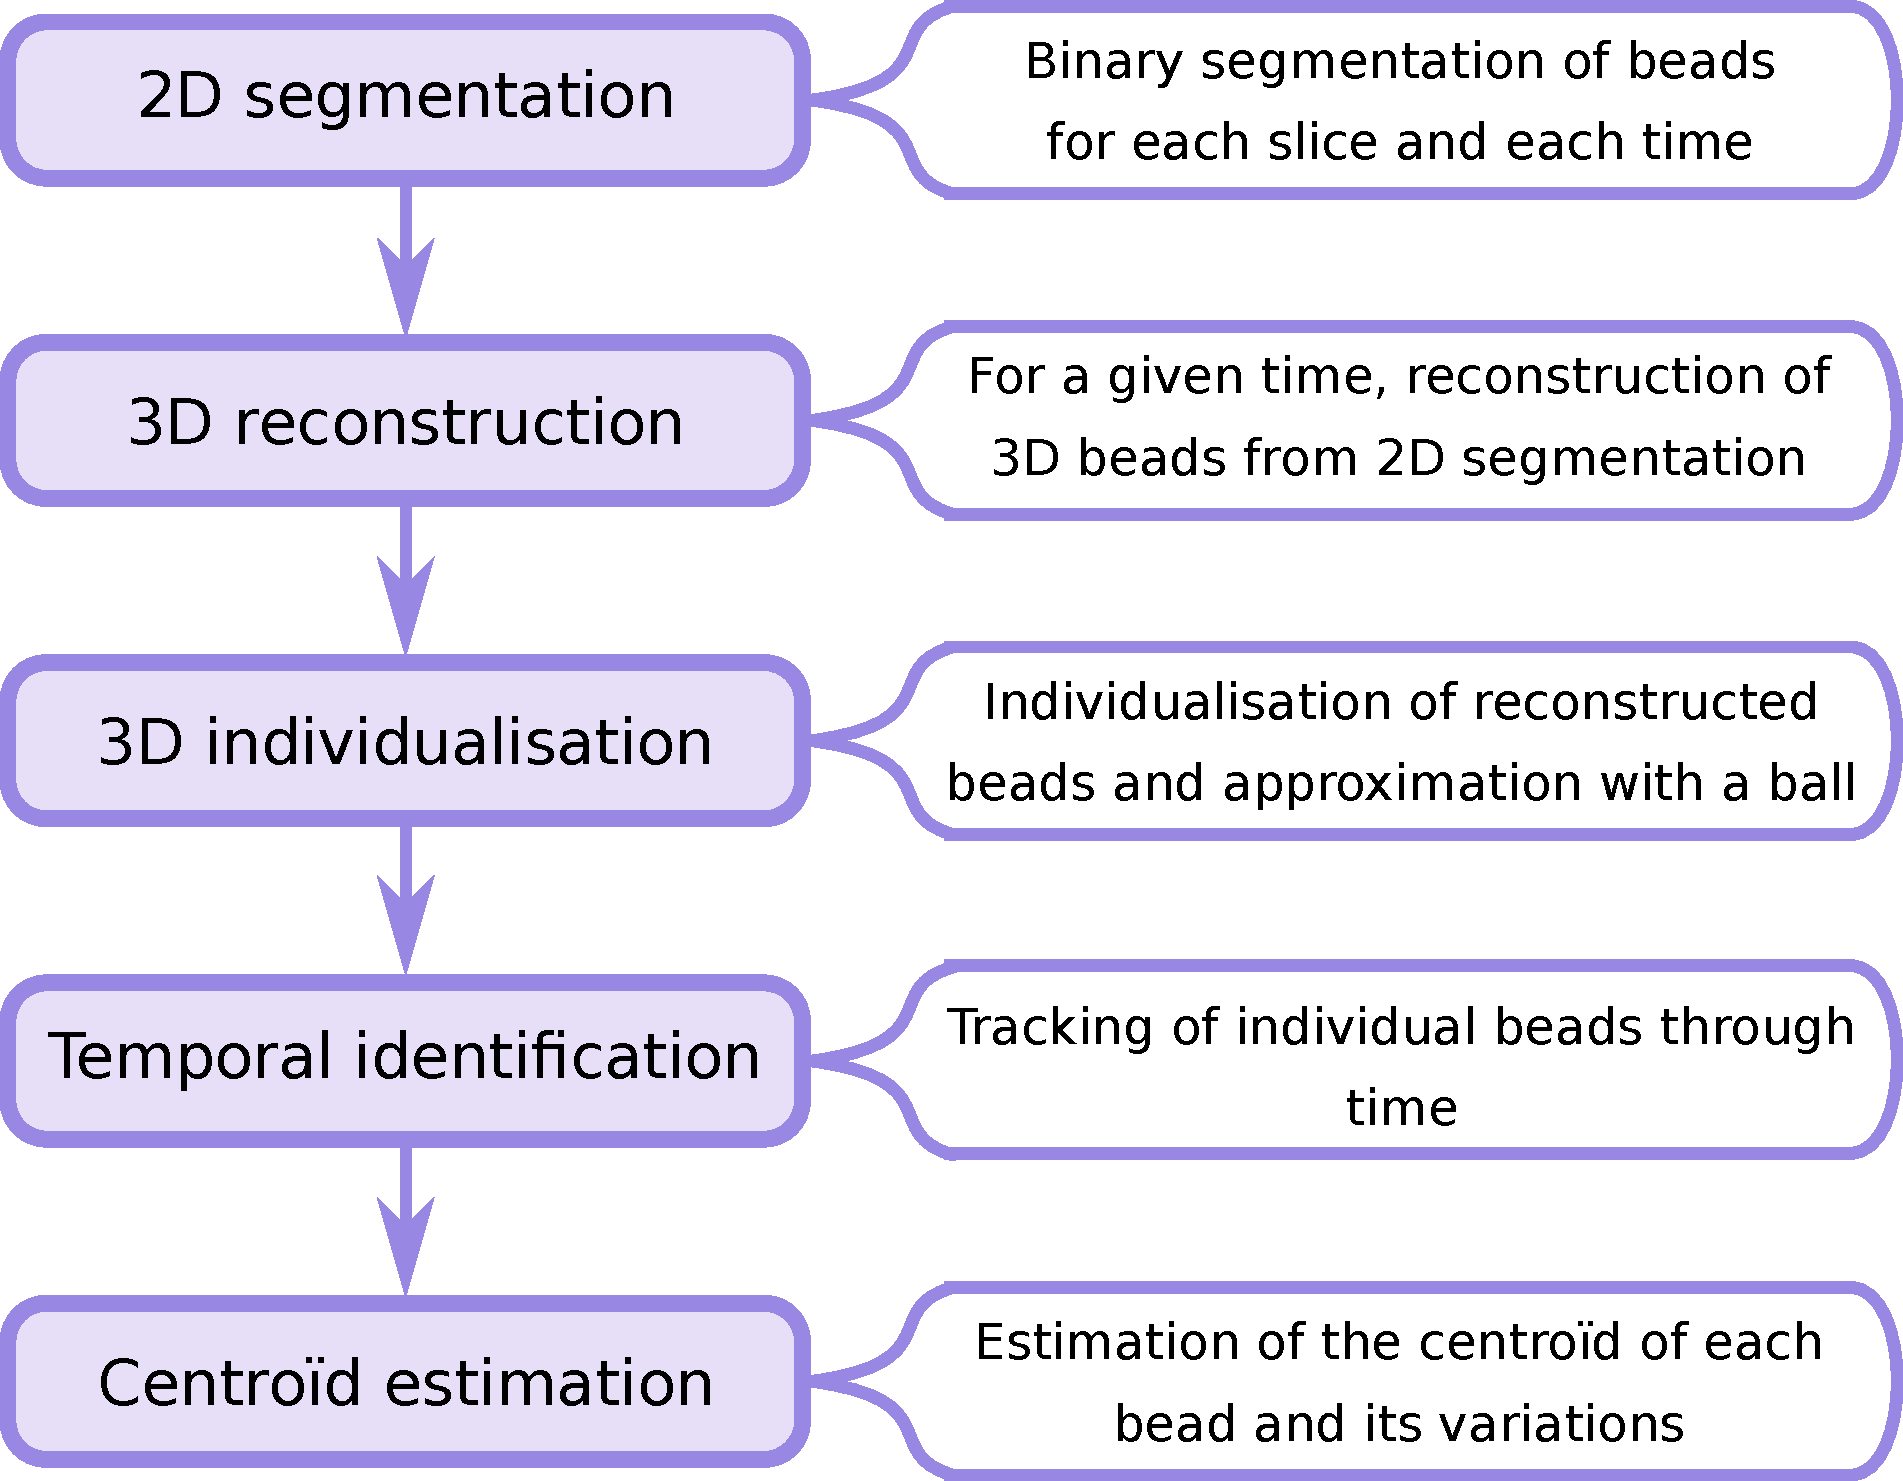
\includegraphics[width =  0.8\linewidth]{images/flowchart.pdf}
\caption{Flowchart of our pipeline}
\label{fig:flowchart}
\end{figure}

\begin{figure}[hpb]
\centering
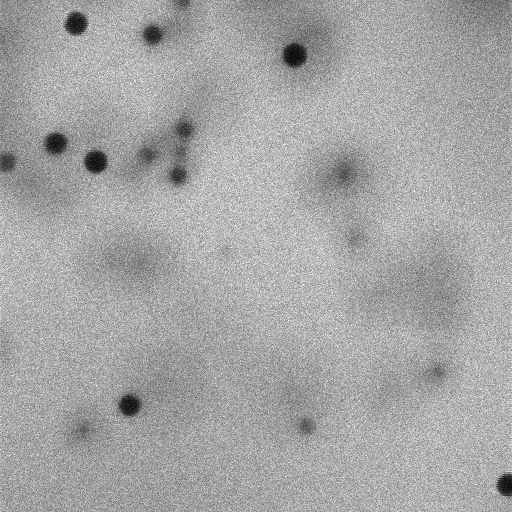
\includegraphics[width =  0.3\linewidth]{images/exp1_t01z1.png}
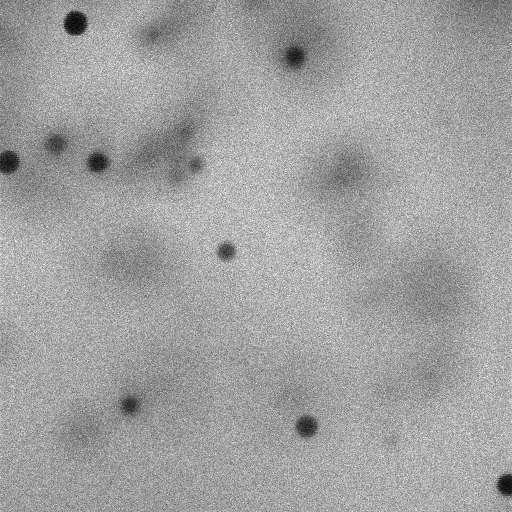
\includegraphics[width =  0.3\linewidth]{images/exp1_t01z2.png}
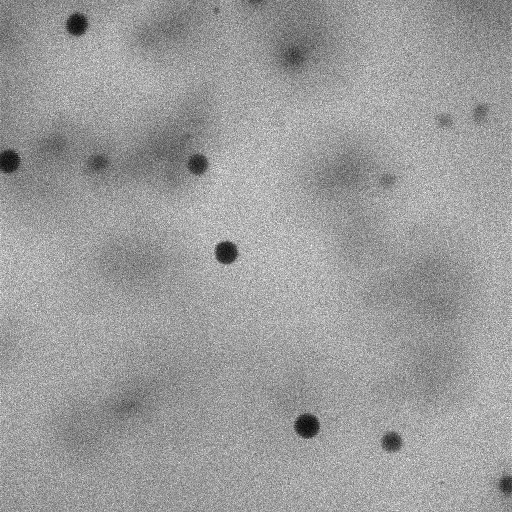
\includegraphics[width =  0.3\linewidth]{images/exp1_t01z3.png}\\
\vspace{0.3em}
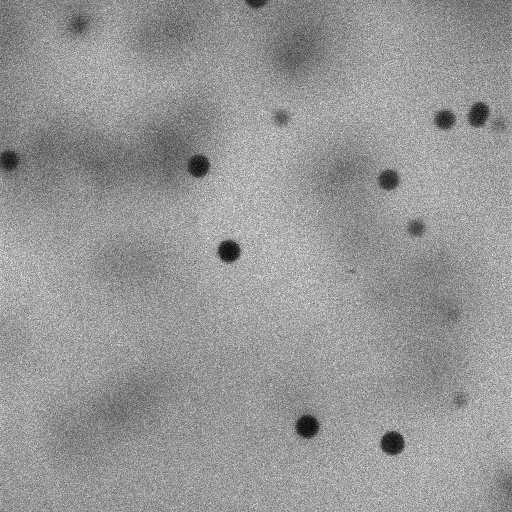
\includegraphics[width =  0.3\linewidth]{images/exp1_t01z4.png}
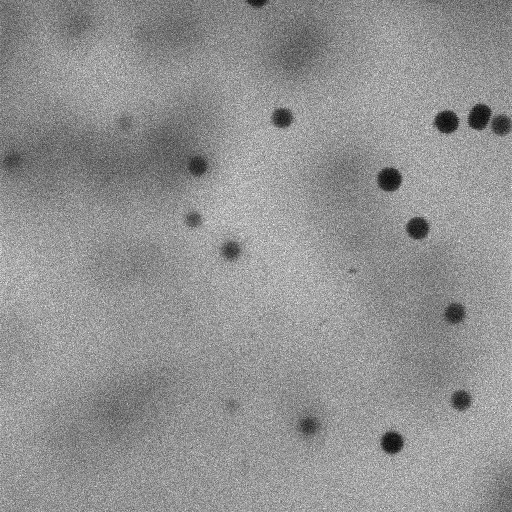
\includegraphics[width =  0.3\linewidth]{images/exp1_t01z5.png}
\caption{Consecutive depth ($z$) slices corresponding to a single time.}
\label{fig:sequence}
\end{figure}

Fig~\ref{fig:flowchart} summarize the pipeline we developed. We named ``2D'' the slices as shown in Fig.~\ref{fig:sequence}. These 5 slices composed the 3D volume for a fixed time.

\subsection{2D segmentation}
The first step of our pipeline is a 2D segmentation of the beads and uses both standard and modern mathematical morphology techniques~\cite{najman-talbot-Wiley-2010}. The objective is to obtain a binary image of the beads suitable for masking and labelling. The steps are the following:
\begin{enumerate}
\item Supression of small local minimas: this is performed using a closing by reconstruction with an initial dilation by a disk of radius 4. This yields image $g$.
\item Calculation of the min-tree of $g$.
\item Filtering of nodes according to multiple criteria: size must be smaller than 500, the grey-level intensity must be lower than 100, and the contrast of the component greater than 80. We keep the maximal components meeting all these criteria.
\item Regularisation of the selected blobs: holes are filled, and the components are dilated with a 4-connected structuring element and opened with a disk of radius 5.
\end{enumerate}
An example of results of this procedure is shown in Fig.~\ref{fig:seg1}

\begin{figure}
\centering
\subfigure[]{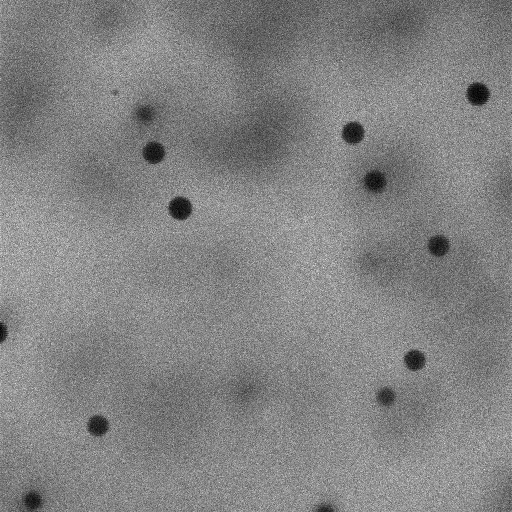
\includegraphics[width =  0.3\linewidth]{images/exp1_t41z4.png}}
\subfigure[]{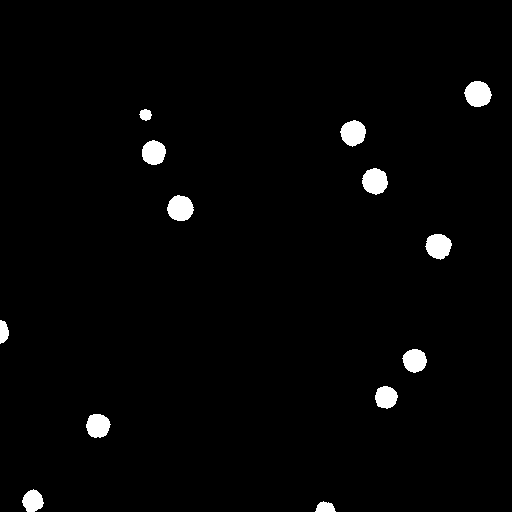
\includegraphics[width =  0.3\linewidth]{images/exp1_t41z4_bin.png}}
\subfigure[]{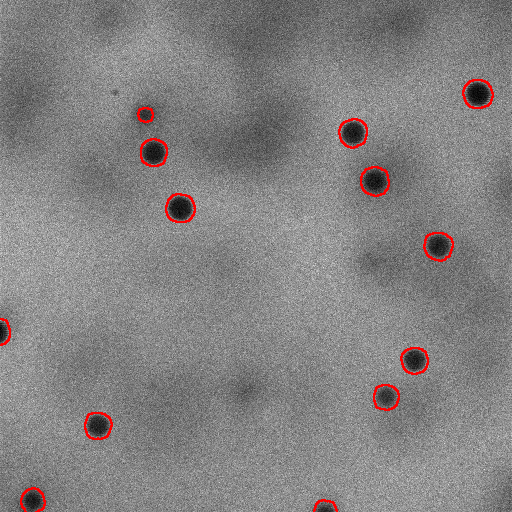
\includegraphics[width =  0.3\linewidth]{images/surimp_exp1_t41z4.png}}
\caption{Illustration of the segmentation procedure: (a) initial image, (b) result of the segmentation described in the text,  (c) overlay of the segmentation on the initial image.}
\label{fig:seg1}
\end{figure}


\subsection{3D regularization}
For each acquisition time, we stack the corresponding 2D segmented slices. As the segmentation is performed in 2D, and the beads may move significantly between slices, some irregularities may appear at the bead boundaries, especially near the bead poles. The first step is hence a regularization in the z axis to reconnect these incomplete beads by applying a 2D closing with a disk of radius 1 in all the $xz$ planes.

\subsection{3D individualization}
As some beads can touch, we separated them using a classical watershed procedure. After noise removal with an opening on the binary image, we extract beads markers using the distance transform with a threshold and the background marker. A watershed is then applied. The result is cleaned by removing small objects using a volume criterion. All the steps are illustrated in Fig.~\ref{fig:temporal}. Morphological parameters were empirically optimized on a small subset of the data.

\begin{figure}
\centering
\subfigure[]{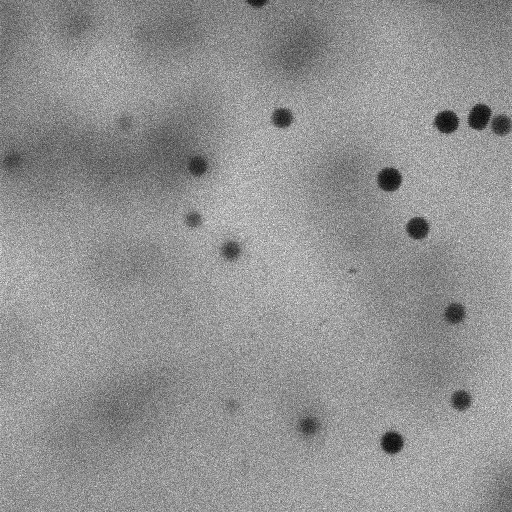
\includegraphics[width =  0.3\linewidth]{images/exp1_t01z5.png}}
\subfigure[]{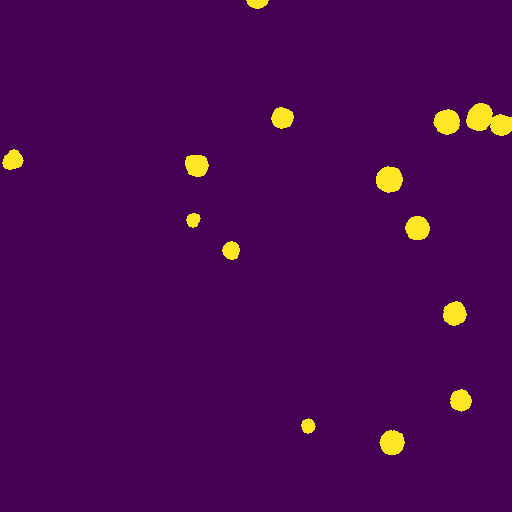
\includegraphics[width =  0.3\linewidth]{images/orig_1.png}}
\subfigure[]{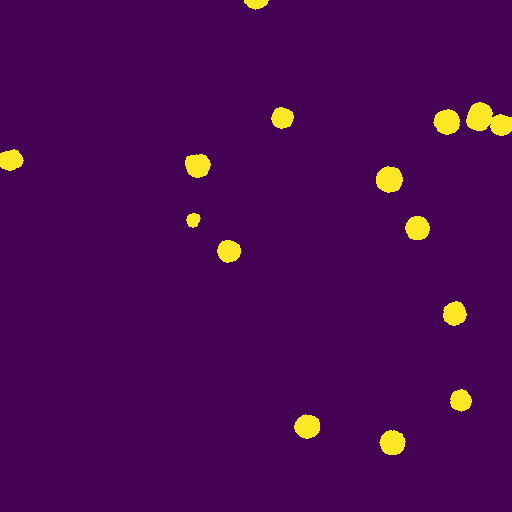
\includegraphics[width =  0.3\linewidth]{images/orig_fermee_1.png}}
\vspace{0.3em}
\subfigure[]{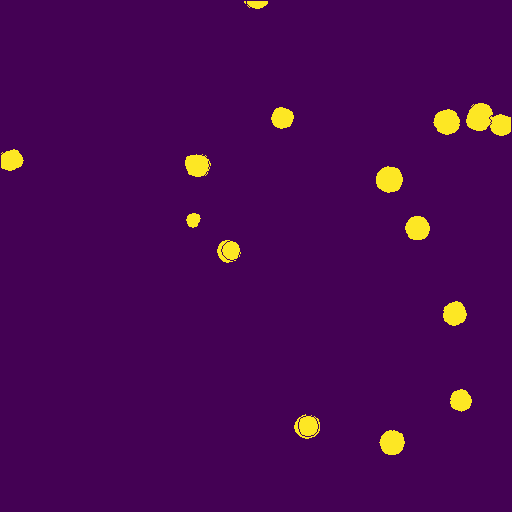
\includegraphics[width =  0.3\linewidth]{images/orig_separ_1.png}}
\subfigure[]{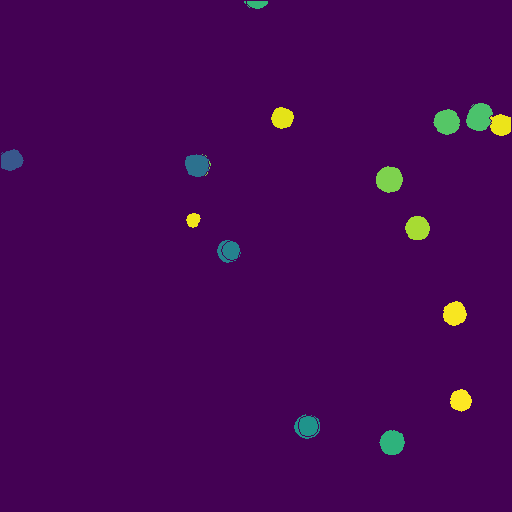
\includegraphics[width =  0.3\linewidth]{images/toto.png}}
\caption{Results of the successive steps: (a) initial image, (b) inital segmentation, (c) 3d regularization, (d) bead separation, (e) individualization and labeling.}
\label{fig:temporal}
\end{figure}
\subsection{Temporal identification}

To label the beads at time $t$, we propagate the labels of the beads at the previous time $t-1$ by finding the intersection between the beads at $t$ and $t-1$. These intersections are the markers used for the reconstruction by dilation. We hence obtain for time $t$ labels for the beads also present at time $t-1$. The remaining unlabeled beads are given new labels. Overall, this procedure is simple but effective, as we will see in the result section.

\section{Position estimation}
In the previous section, 2D bead segmentation is performed and label clustered in 3D. We consequently assume that a uniquely labeled object in 3D constitutes a single bead.

Estimating the 3D position of each bead from their 2D slice is a challenge. We propose to estimate 2D positions first, and derive the 3D position from an estimation of the radius of the bead.

\subsection{Centroid estimation in 2D}
Various methods can be used to estimate the centroid of a disk. A least-square best-fit disk can for example be used~\cite{gander1994least,fitzgibbon1999direct}. However these methods are more appropriate when only a subset of the disk contour is known. Since the beads are small, we can assume that most of them do not lie near the border of the field of view, and so are totally visible. In this case, a moments-based method seems more appropriate~\cite{hu1962visual}. Let $M_{pq}$ be a moment of order $p+q$ defined as follows:
\begin{equation}
M_{pq} = \sum_x\sum_y x^p y^q I(x,y),
\end{equation}
where $I(x,y)$ is the intensity of the image at position $x,y$. If we restrict $I(x,y)$ to be equal to 1 for the segmented bead with label $l$ and 0 elsewhere, then 
\begin{equation}
\bar{x}_l = \frac{M_{10}}{M_{00}} \;\;;\;\; \bar{y}_l = \frac{M_{01}}{M_{00}},
\end{equation}
yield the coordinates of the centroid of bead $l$. Moments of order 0 and 1 are not affected by isotropic blur or partial volume effects and are relatively resistant to noise, and so this estimation is rather robust, as we will see later in simulations. Moreover, we can also estimate the radius via the second order centered moments
\begin{equation}
\mu_{20} = M_{20} - \bar{x}M_{10} \;\;;\;\; \mu_{02} = M_{02} - \bar{y}M_{01},
\end{equation}
and then for a disk $\mu_{20}=\mu_{02} = \frac{\pi}{8}r^4$, or more simply from the disk area equation $r=\sqrt{M_{00}/\pi}$.

\subsection{Centroid estimation in 3D with known bead radius}
If we know the radius $R$ of a bead to a good precision, we can estimate the depth $p_R$ by noting that
\begin{equation}
p_R = \pm\sqrt{R^2-r^2},\label{eq:depth}
\end{equation}
with $r$ the estimated radius of the disk, as seen on Fig.~\ref{fig:depth}

\begin{figure}
\centering
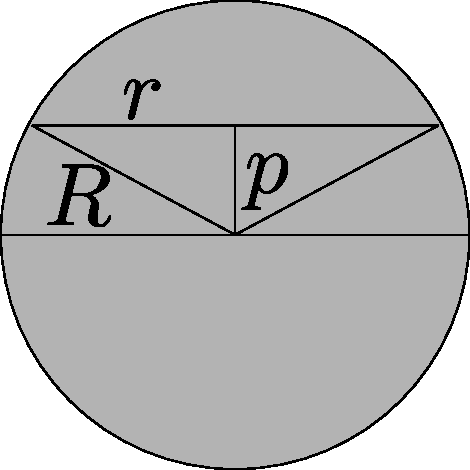
\includegraphics[width=0.3\textwidth]{images/depth.pdf}
\caption{Bead depth estimation: $R$ is the real radius, $r$ the observed radius, and $p$ the estimated depth.}
\label{fig:depth}
\end{figure}
Unfortunately there is a sign uncertainty with this estimation, so a correct estimation must include information from the other slices associated with the same bead. Fig.~\ref{fig:multidepth} illustrates what happens, in a 2D $x+z$ simplified setting. Each intersection between the bead and a scanning plane yields a disk (a line in the drawing), from which two depths can be estimated,  only one of which is correct. The beads is moving between acquisitions, so there are two depths estimations per slice. We assume the correct ones are those that minimize the overall distance between them.

\begin{figure}
\centering
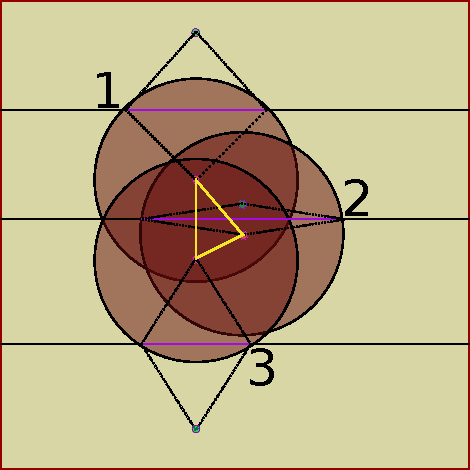
\includegraphics[width=0.5\textwidth]{images/multidepth.pdf}
\caption{When estimating the depth of the bead centroid over multiple slice acquisition (labeled 1, 2 and 3 in the drawing), as the bead is moving during the acquisition, the centroid depth varies and can be one of two possibilities. We select the depth estimations that minimizes the overall Euclidean distance between them (i.e. corresponding to the perimeter of the yellow triangle).}
\label{fig:multidepth}
\end{figure}

More formally, for every slice $s$, for every bead with label $l$ we estimate two centroid positions 
\begin{align}
c_s^{l,0} &= (\bar{x}_l, \bar{y}_l, d(s)-p_R(s)) \label{eq:cs0}\\ 
c_s^{l,1} &=  (\bar{x}_l, \bar{y}_l, d(s)+p_R(s))\label{eq:cs1},
\end{align} 
with $d(s)$ the depth of slice $s$ and $p$ given by~\eqref{eq:depth}. For every slice $s$ we have two choices.  If $v \in \{0,1\}^{n_s}$ is a binary vector of length $n_s$, the total square distance is 
\begin{equation}
d_{v,R}^2 = \sum_{s=0}^{n_s-1} \|c_s^{l,v[s]}-c_s^{l,v[(s+1)\text{ mod } n_s]}\|^2,\label{eq:dv}
\end{equation}
where $a \text{ mod } b$ is the remainder of the integer division of $a$ by $b$, and assuming without loss of generality that slices are numbered 0 to $n_s-1$.

We propose to select the vector $v$ corresponding to the combination that minimizes $d_v$. Consequently, if there are $n_s$ slices for a bead,  we need to test $2^{n_s}$ combinations.
In our experiments, we have 3-6 slices for each bead, meaning up to 64 tests per bead, which is manageable. If we had more slices, this could be a problem. In this case, a simplification would be to select the middle slice, and for both centroid estimations related to this slice, compute the distance to the two centroid position estimations to every other slides. In other words we now minimize $d_{v,R}'^2$ defined as follows:
\begin{equation}
d_{v,R}'^2 = \sum_{s=0}^{n_s-1} \|c_s^{l,v[s]}-c_s^{l,v[\floor*{n_s/2}]}\|^2,\label{eq:dprime}
\end{equation}
where $\floor*{a}$ is the integer part of $a$. The difference here is that each term of this sum can be minimized independently, and so there are only $4 n_s$ combinations to test, which is beneficial as soon as $n_s \geq 4$.

\subsection{Centroid estimation in 3D with imprecise bead radius}
If the radius is not known precisely and varies from bead to bead, which is often the case, the problem is more difficult. We assume that the bead radius  for each bead is a deviate from a known Gaussian distribution of mean $\bar{R}$ and standard deviation $\sigma_R$. Typically, $\sigma_r \approx 0.1\bar{R}$.
\begin{equation}
R_l \sim G(\bar{R}, \sigma_R)
\end{equation}
Given the known observations for each bead, we also know that $r_l$ is greater than the largest measured radius $r_{\text{max}}=\max\{r_s, s\in \Iintv{0,n_s-1}\}$. We solve the following mixed problem:
\begin{align}
R^*_l,v^* &= \argmin_{R,v} d_{v,R}^2 + \frac{1}{2\lambda} \|R-\bar{R}\|^2 \label{eq:opt}\\
\text{s.t.}&\; R \geq r_{\text{max}}.\label{eq:constr},
\end{align}
where $\lambda$ is a Lagrangian parameter, and the second term of~\eqref{eq:opt} is the log-likelihood of a Gaussian distribution for $R$, thus we expect $\lambda$ to be proportional to $\sigma_R^2$. The tighter the distribution, the more important this term becomes.

For a given $v$ binary vector,~\eqref{eq:depth} is convex due to the constraint~\eqref{eq:constr}, the constraint itself is linear since $r_{\text{max}}$ is an observation, but both~\eqref{eq:dv} and \eqref{eq:dprime} are smooth differences of convex functions, so this problem cannot be solved by standard constrained convex optimisation methods~\cite{boyd2004convex}. However, it can be tackled by DC methods~~\cite{tao2005dc}. In addition, the problem remains combinatorial in $v$, as seen above, so we need to run several such DC problems, up to $2^{n_s}$ or $4n_s$ depending on whether we choose to optimise~\eqref{eq:dv} or \eqref{eq:dprime}. 

Since DC method solvers are complex to handle, we propose to solve~\eqref{eq:opt} using gradient descent with the $d'$ measure of~\eqref{eq:dprime}, but taking as reference the slice with the largest measured radius $r_{\max}$ instead of the middle slice. We set $\max\{r_{\max}, \bar{R}\}$ as the initialization for $R$ and $\lambda=\sigma_R$. In practice, the true $R^*$ is very close to the largest observed radius.

\section{Results on simulations}
To test our method, we simulate $N$ discrete sphere beads at high resolution with a random radius sampled from a Gaussian distribution as described in the previous section. The beads are subjected to isotropic Brownian motion and depth-ordered slice acquisition. We down-sample the result to ensure sub-pixel accurate positions. We estimate the radius of the intersection disk between each slice and the bead via the area method, and the $\bar{x}$, $\bar{y}$ position via moments. 
The $z$ position and the bead radius is estimated as described above using the $d'$ method.

\begin{figure}
\centering
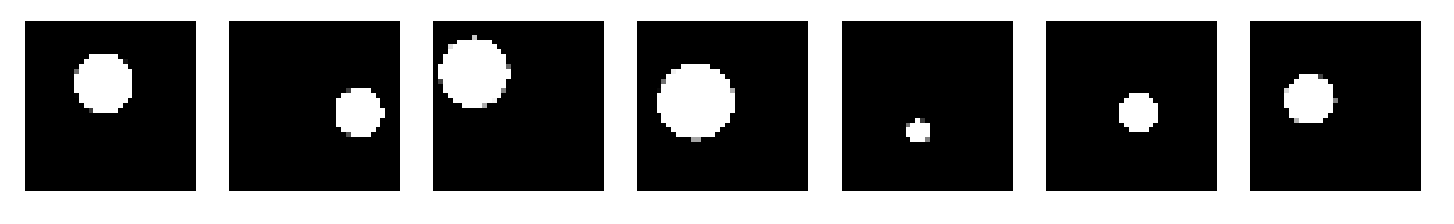
\includegraphics[width=0.5\textwidth]{images/simulated.png}
\caption{A single simulated bead acquired over several layers subjected to Brownian motion.}
\label{fig:simulated_beads}
\end{figure}

For this simulation, we simulate high-resolution beads 80 pixels in radius, in a $350^3$ cube, acquired through 7 layers and subjected to  Brownian motion with an isotropic diffusion coefficient of 0.1 relative to the size of the cube, or 35 pixels at high resolution. Low resolution images were down-sampled by a factor of 10 with nearest-neighbor interpolation. The diffusion coefficient of the Brownian motion can be interpreted as the standard deviation of the the components of the position of the center of the bead from one slice to the next. With Brownian motion, the average deviation is zero.

Figure~\ref{fig:simulated_beads} shows the intersection of a single bead through successive slices. The Brownian motion influence is significant and clearly seen. We simulated 100 beads, which generated 540 slices. Via our optimisation procedure, each slice provides a 3D center estimate from which various measurements can be derived. In particular, we compare the estimation of the center position to the simulated ground truth. The results are shown in Table~\ref{tab:rel_error}

\begin{table}[htb]
\centering
\caption{Positional RMS relative error}
\begin{tabular}{|c|c|c|c|}\hline
                & $x$            & $y$            & $z$ \\\hline
Relative error  & $1.6\;10^{-3}$ & $1.6\;10^{-3}$ & $8.2\;10^{-3}$ \\\hline
\end{tabular}
\label{tab:rel_error}
\end{table}

On this table, we see that the average Euclidean position error in $x$ and $y$ is very low. Indeed, a pixel error in 350 (the high-resolution size of the cube) would translate into $2.8\;10^{-3}$. However, the $z$ estimation error is 5$\times$ greater, which is still sub-pixel accurate at the low sub-sampled resolution, and so still quite acceptable. We note that these estimates are the same as our estimate of the average Brownian deviation, which should be zero.

\begin{figure}
\centering
\subfigure[]{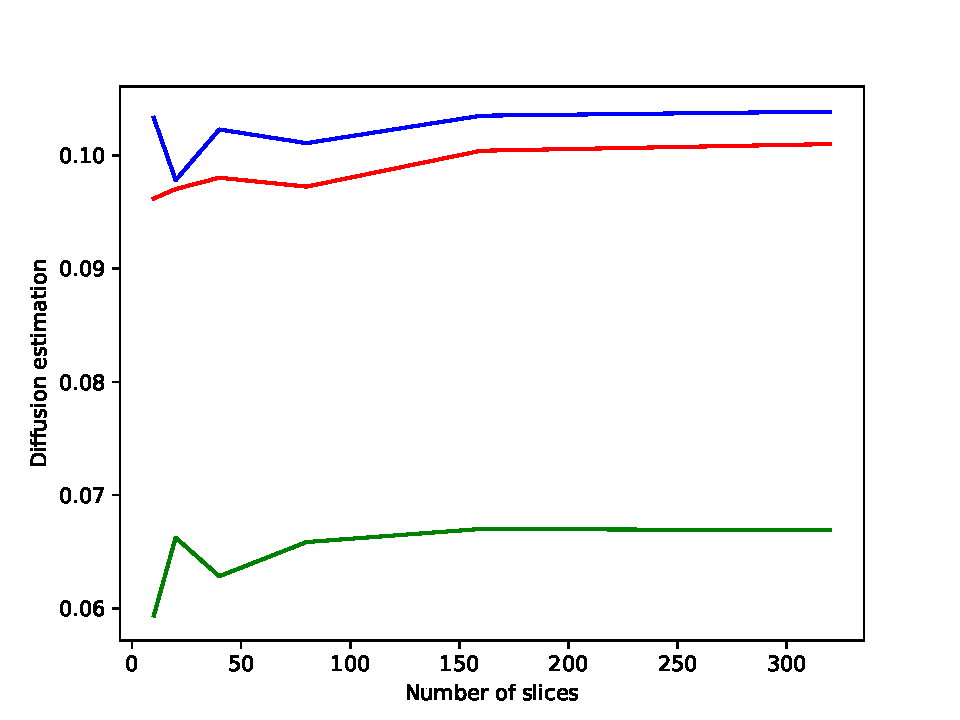
\includegraphics[width=0.45\textwidth]{images/ave_vs_smpl.pdf}}
\subfigure[]{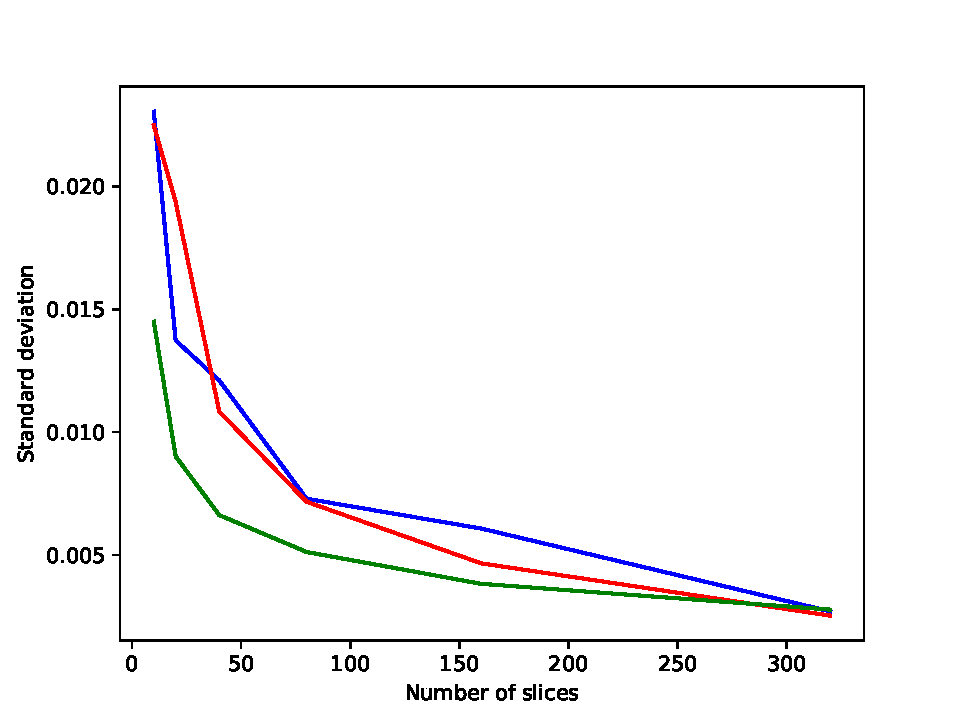
\includegraphics[width=0.45\textwidth]{images/std_vs_smpl.pdf}}
\caption{Convergence of the diffusion estimator to a stable value (a) and its standard deviation as a function of the number of slices (b).}
\label{fig:estim}
\end{figure}

On Fig.~\ref{fig:estim}, we show the estimation of the relative Brownian diffusion coefficient as a function of the sample size. We expect a relative
coefficient of $10^{-1}$, i.e. the one we simulated. The $x$ and $y$ are very close to this estimate, but the $z$ diffusion estimation appears biased with a value about 70\% as much as it should be. All three estimators converge quickly and can be deemed reliable from about 50 slices, i.e. 10 beads or so, with a standard deviation of the estimate of diffusion coefficient close to $10^{-2}$, ie. 10\% error. With 40 beads, or 200 slices, the standard deviation of the diffusion coefficient drops down to $5\;10^{-3}$ or 5\% relative error.

Currently, this means that our optimisation method is indeed good enough for positional estimation in 3D, but that for more subtle measurements, like diffusion coefficient estimations, 2D measurements are sufficient. We note that we are able to measure this diffusion coefficient from single 3D acquisition only.

\section{Results on real data}
We applied our method on a video of 3$\mu$m beads, with $\Delta t=0.5s$. Resolution is $0.125\mu\text{m}$ per pixel in $x$ and $y$, and only $0.5\mu\text{m}$ per slide in $z$. Comparison with manual labelling results show that we manage to correctly detect and label all beads, as well as track each bead individually with zero label error between 3D volumes. However, we overestimate beads presence in the z-axis due to the point spread function (PSF) of the microscope. In practice this means that beads faintly appear in slices above and below their true position. This overestimation is depicted in Fig.~\ref{fig:compa}(c). On slice 0, we tend to find beads that are not supposed to be segmented (false positives), i.e.the central bead of the illustration. This ``oversegmentation'' is nonetheless acceptable as it remains coherent in 3D and does not imply bias in 2D. In 3D, this can cause the bead radius to be overestimated, and will need to be corrected in future work.

\begin{figure}
\centering
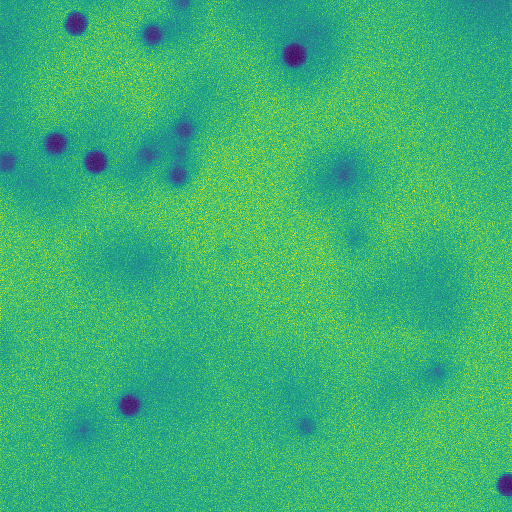
\includegraphics[width = 0.3\linewidth]{images/orig_tot.png}
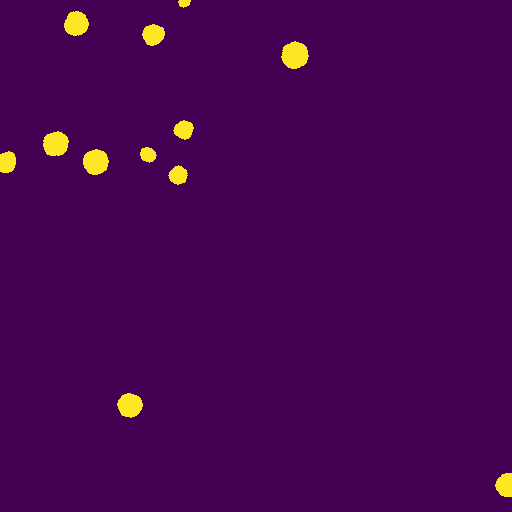
\includegraphics[width = 0.3\linewidth]{images/seg_base_tot.png}
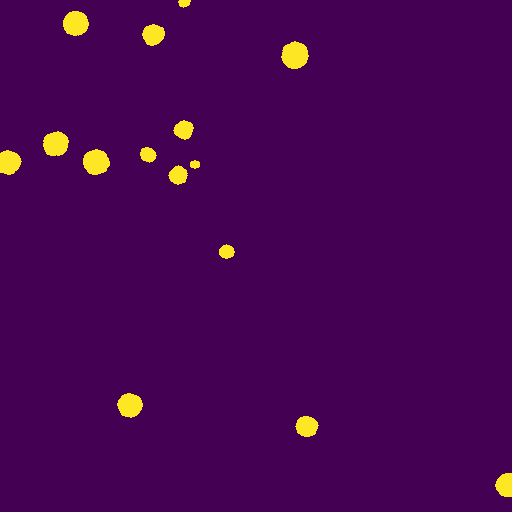
\includegraphics[width = 0.3\linewidth]{images/modif_tot.png}\\
\vspace{0.3em}
\subfigure[]{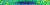
\includegraphics[width = 0.3\linewidth]{images/orig.png}}
\subfigure[]{
\includegraphics[width = 0.3\linewidth]{images/seg_base.png}}
\subfigure[]{
\includegraphics[width = 0.3\linewidth]{images/modif.png}}\\
\caption{Comparison of segmentation results: (a) original frame, (b) results of the first step of the 2D segmentation procedure before regularization, and (c) after 3D regularization. Top images are the entire $xy$ slices, and the bottom is a $xz$ view along the z-axis}
\label{fig:compa}
\end{figure}

On this sample, using our 2D method, we estimate an average diffusion coefficient of $4.3\;10^{-2}$ relative to the beads average diameter. Currently we do not have the ground truth for this measurement. 

\section{Conclusion}\label{sec:Conclusion}
In this article we tacked the problem of tracking fluorescent beads in 
confocal microscopy, when we do not assume that beads are small enough to be assimilated to point sources, but instead span several slices; when they move between slices due to Brownian motion; and when their radius is not precisely known. Starting from 2D-based segmentation and 3D clustering using shape-based mathematical morphology, we have shown that estimating bead radius and true 3D positions from a small number of 2D slices is a difficult, but tractable problem. We have also shown that tracking these beads between 3D acquisitions is possible with a high degree of accuracy. One benefit of our approach is that we can obtain good estimates of the diffusion coefficient of Brownian motion from single 3D acquisition, which is useful for various physical measurements.

In future work, we plan to improve the quality and speed of our optimisation method, to make better use of prior knowledge in 3D particularly for initial segmentation, and we will release our software as a free, open-source package.

\bibliographystyle{splncs04}
\bibliography{tracking3d}


\end{document}

